\section{Projektplan für die Bachelor-Arbeit}
Der Zeitplan für die Bachelor-Arbeit ist in Abbildung \ref{img:terminplan} auf Seite \pageref{img:terminplan} dargestellt.
Im oberen Teil sind die allgemeinen Termine und Abwesenheiten aufgeführt. Der mittlere Teil zeigt die Arbeitsverteilung über das Semester und am Schluss kommen die Zeitaufwände für Doku und Meetings. Die Dokumentation wollen wir kontinuierlich erstellen, sodass wöchentlich ein entsprechender Block vorgesehen ist.
% Abbildung (A3)
\newpage
\clearpage
\pagebreak
\afterpage{ % Insert after the current page
\clearpage
\KOMAoptions{paper=a3, paper=landscape} 
\recalctypearea

\begin{figure}[htbp]
	\centering
	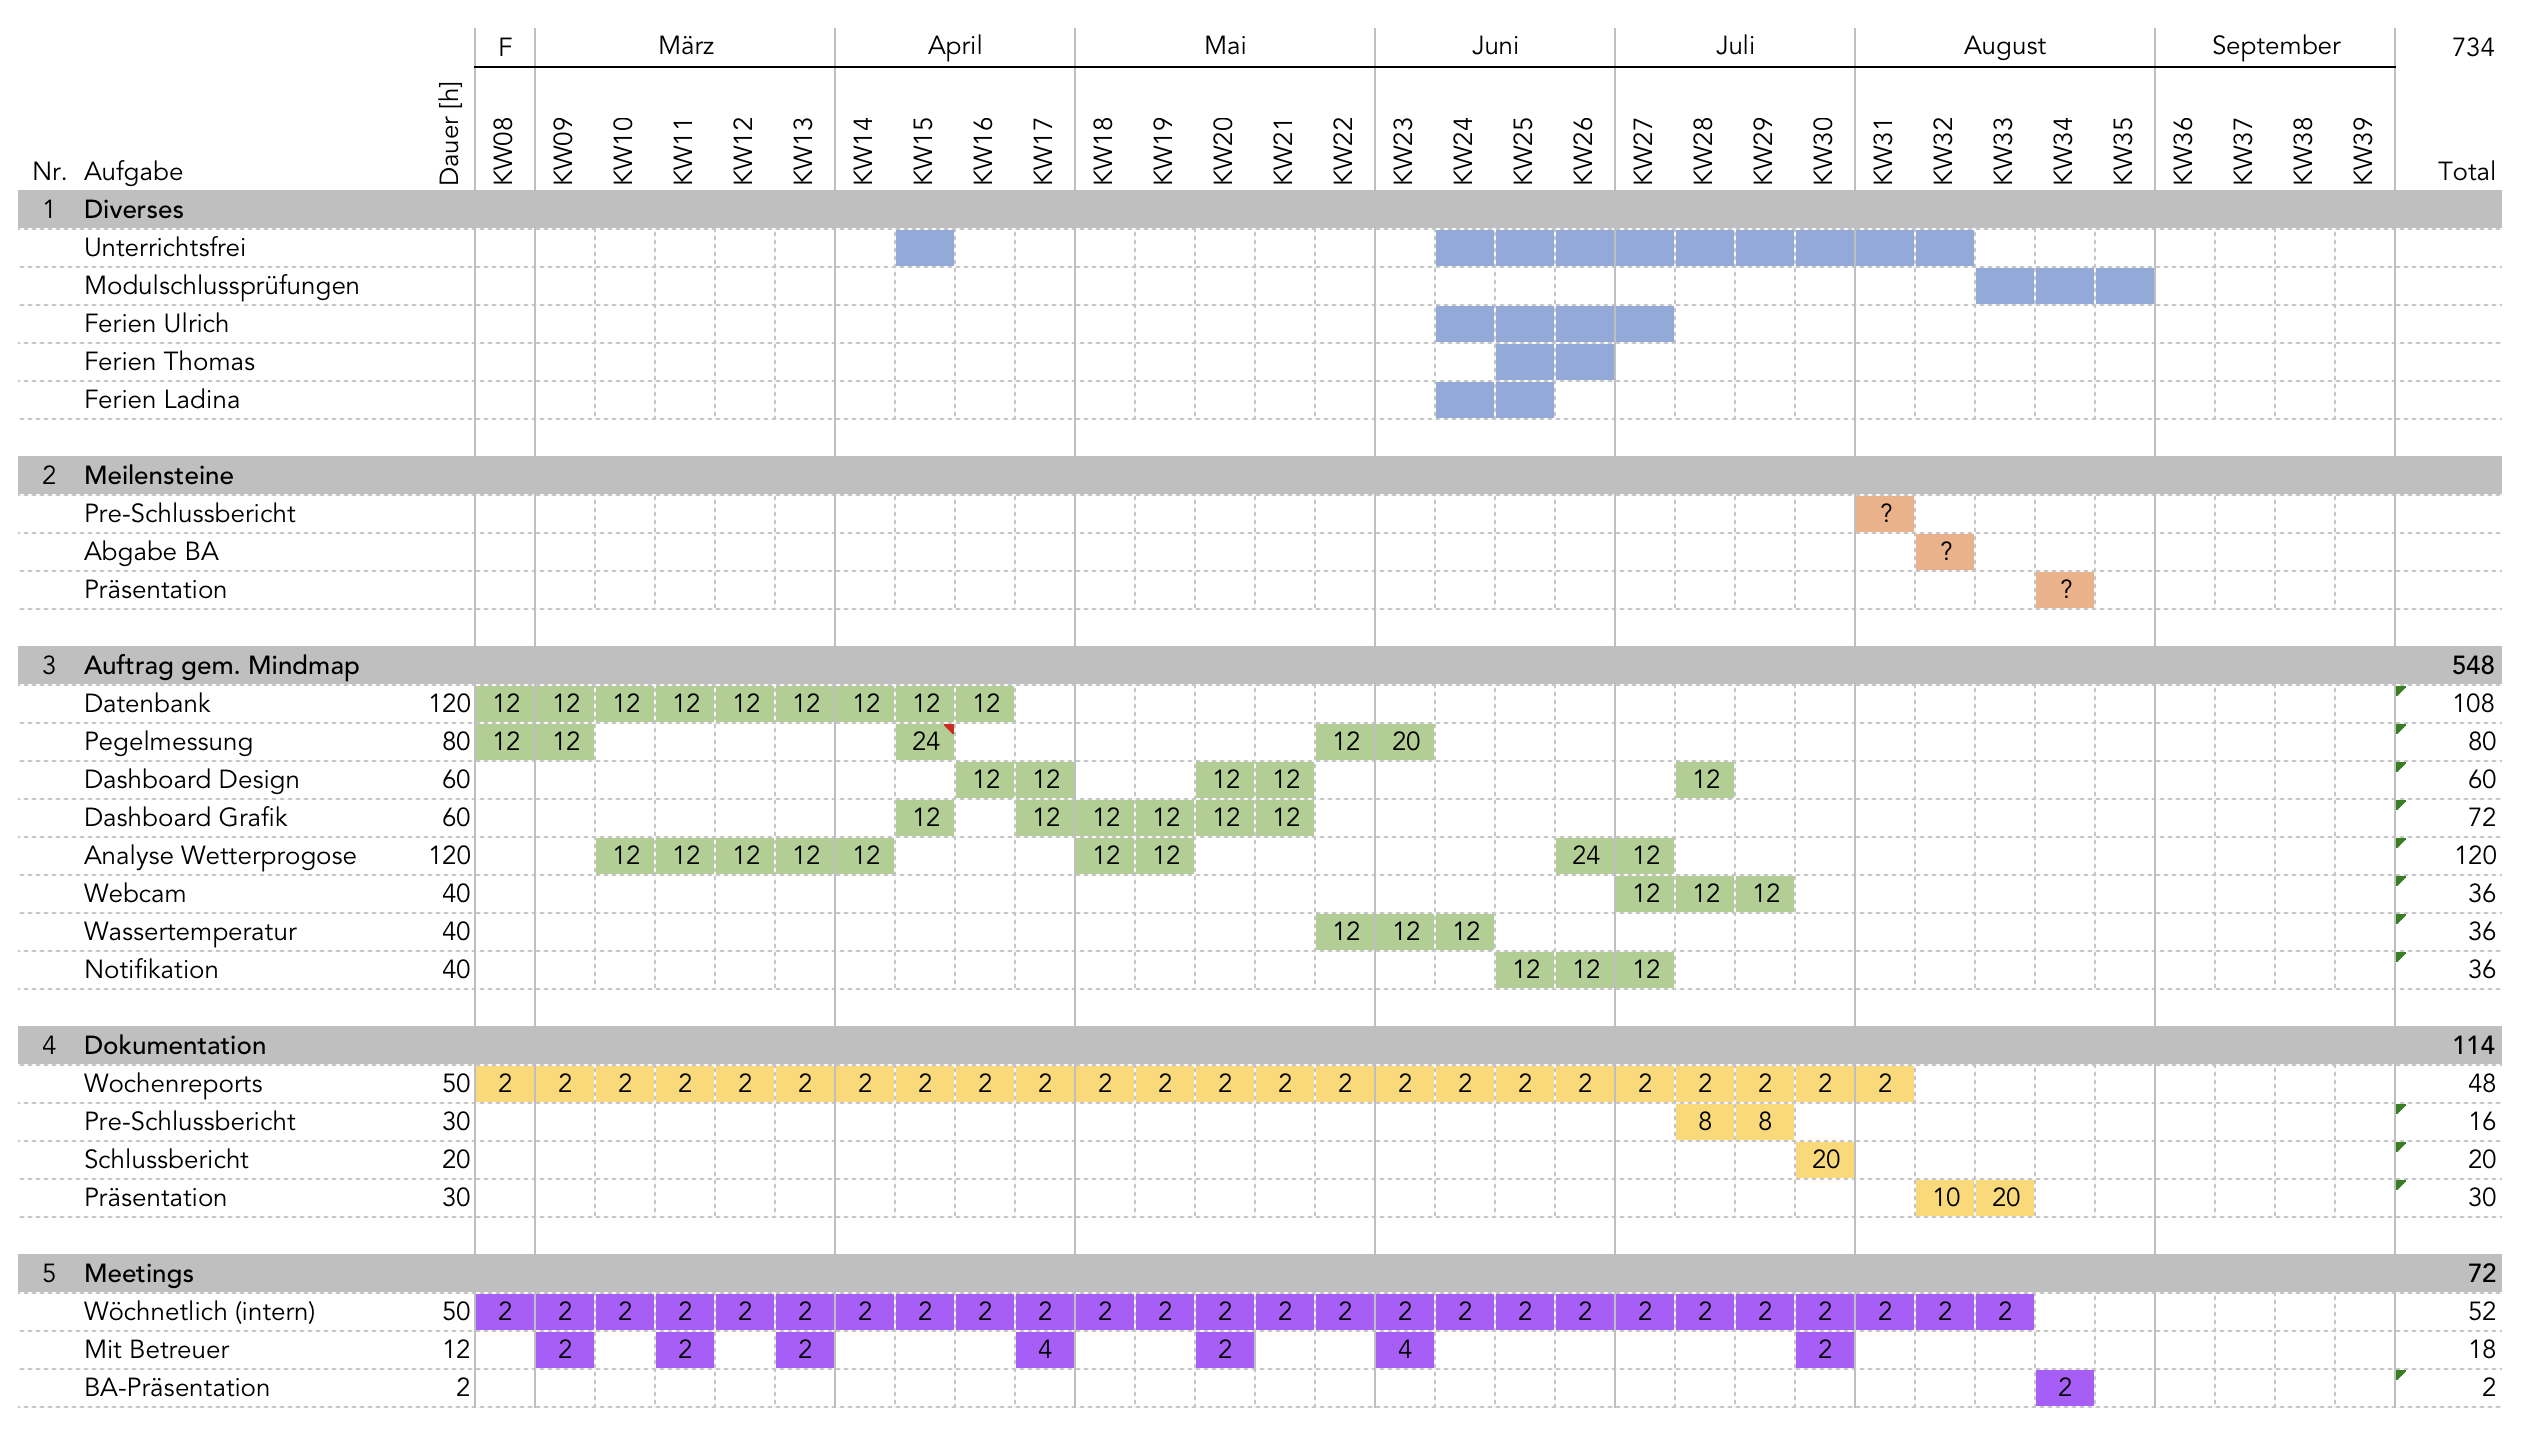
\includegraphics[width=1.1\linewidth]{img/terminplan} % ab heigth = 0.6 auf eigener Seite!
	\caption{Terminplan}
	\label{img:terminplan}
\end{figure}
\clearpage
\KOMAoptions{paper=A4,pagesize}
\recalctypearea
}
